% # To do
% - show eigendecomposition of the covariance matrix minimizes the projection residuals
% - minimizing projection residuals maximizes variance
% - SVD
% - PCA algorithm
% - Fix notation in PCA example

% rewrite this paragraph to focus on minimizing projection residuals
Principal component analysis (PCA) is a coordinate transform that minimizes projection residuals along each of the major axes \(v_1, v_2, \dots, v_d\) of the transformed space.
These axes are referred to as \textit{principal components}.
After the PCA transform is applied to a set of observations, the smallest projection error is along the first principal component.
If we project down to two dimensions, the first two principal components have the smallest projection error.
In general, projecting down to \(p \leq d\) dimensions is most accurate along \(v_1, v_2, \dots, v_p\).

Conversely, projecting along \(v_2, \dots, v_d\) will result in the largest residual error in \(d-1\) dimensions.
It follows that \(v_1\) must be the direction with the highest variance.
Then \(v_2\) is the direction with the next highest variance, and so on.

\subsection{Minimizing projection residuals}

% derive the first principal component by minimizing the projection residual
% derive the next principal component orthogonal to the first one that minimizes the projection residual



% lead into the algorithm

\begin{algorithm}
    \everymath{\displaystyle}
    \caption{Principal component analysis}
    \label{alg:principal-component-analysis}
    \KwIn{Data matrix \(A \in \RR^{n \times d}\) and number of components \(p \leq d\)}
    \KwOut{Coefficient matrix \(V_p \in \RR^{d \times p}\) and transformed data \(\tilde{A} \in \RR^{n \times p}\)}

    \tcp{Center the data}
    \(A_0 \gets A - \colmean(A)\)\;

    \tcp{Compute \(d \times d\) covariance matrix}
    \(C \gets \frac{1}{n-1} A_0^\top A\)\;

    \tcp{Diagonalize covariance matrix \(CV = VD\)}
    \([V, D] \gets \operatorname{eig}(C)\)
    where \\[4pt]
    \(V = \begin{bmatrix}
        v_1, & v_2, & \dots, & v_d
    \end{bmatrix}\)
    such that \(v_1, v_2, \dots, v_d \in \RR^d\) and \\[4pt]
    \(D = \operatorname{diag}(\lambda_1, \lambda_2, \dots, \lambda_d)\)
    such that \(\lambda_1 \geq \lambda_2 \geq \cdots \geq \lambda_d\)\;

    \tcp{Reduce dimension}
    \(V_p \gets \begin{bmatrix}
        v_1, & v_2, & \dots, & v_p
    \end{bmatrix}\)\;

    \tcp{Transform data}
    \(\tilde{A} \gets A_0 V_p\)\;
\end{algorithm}

\begin{example}
    \def\Amat{\begin{bmatrix}
        5 &  3 &  6 &  7 &  6 \\
        4 &  5 &  7 &  1 &  3 \\
        5 &  7 &  6 &  1 &  0 \\
        6 & 10 & 12 & 12 & 11 \\
        9 & 10 & 12 & 13 &  9 \\
    \end{bmatrix}}
    Consider the following matrix \[A = \Amat.\]
    The column means are \(\mu = [5.8,7,8.6,6.8,5.8]\).
    Then the mean-centered data becomes
    \def\-{\phantom{-}}
    \[X = A - \mu = \frac{1}{5}\begin{bmatrix}
            -4 &   -20 &   -13 &   \-1 &   \-1 \\
            -9 &   -10 &    -8 &   -29 &   -14 \\
            -4 &   \-0 &   -13 &   -29 &   -29 \\
            \-1 &  \-15 &  \-17 &  \-26 &  \-26 \\
        \-16 &  \-15 &  \-17 &  \-31 &  \-16 \\
    \end{bmatrix}.\]

    The covariance matrix is
    \[C = X^TX = \frac{1}{5}\begin{bmatrix}
            74 &  85 &  93 & 179 & 104 \\
            85 & 190 & 170 & 225 & 150 \\
            93 & 170 & 196 & 313 & 238 \\
        179 & 225 & 313 & 664 & 484 \\
        104 & 150 & 238 & 484 & 394 \\
    \end{bmatrix}.\]
    
    Diagonalizing \(C\) gives
    \begin{align*}
        V &= \begin{bmatrix}
            0.1888 & -0.2020 & -0.6366 &  0.5495 & -0.4651\\
            0.2755 & -0.7886 &  0.1472 & -0.4502 & -0.2791\\
            0.3606 & -0.3464 &  0.3128 &  0.5836 &  0.5582\\
            0.6979 &  0.2522 & -0.4422 & -0.3707 &  0.3411\\
            0.5209 &  0.3922 &  0.5288 &  0.1316 & -0.5271\\
        \end{bmatrix},\\
        D &= \begin{bmatrix}
            264.8458 &       0 &      0 &      0 & 0 \\
                    0 & 27.9766 &      0 &      0 & 0 \\
                    0 &       0 & 9.3198 &      0 & 0 \\
                    0 &       0 &      0 & 1.4579 & 0 \\
                    0 &       0 &      0 &      0 & 0 \\
        \end{bmatrix}.
    \end{align*}
    
    If we keep all \(5\) principal component vectors, then \(V_5 = V\) and the projection of \(X\) along \(V\) is
    \[P = XV = \begin{bmatrix}
        -1.9469 &  4.3453 & -0.8756 & -0.2039 & 0 \\
        -6.9742 & -0.0660 &  1.4352 &  0.7590 & 0 \\
        -8.1577 & -2.6752 & -0.8063 & -0.5704 & 0 \\
            8.4282 & -0.2330 &  1.8282 & -0.4996 & 0 \\
            8.6507 & -1.3711 & -1.5815 &  0.5149 & 0 \\
    \end{bmatrix}.\]
    Here, the last column of \(P\) is the zero vector because the last eigenvalue of \(C\) is zero\footnote{Since we subtracted the column means from a square matrix \(A\), the dimension of the row space was reduced to 4.}.
    To perfectly reconstruct \(A\), we need \(k = 4\) principal components and the row vector \(\mu\)
    \[A = PV^T + \mu = PV_4^T + \mu.\]
    
    If we use \(k = 3\) principal components, then the projection of \(X\) onto \(V_3\) is
    \[P = XV_3 = \begin{bmatrix}
        -1.9469 &  4.3453 & -0.8756 \\
        -6.9742 & -0.0660 &  1.4352 \\
        -8.1577 & -2.6752 & -0.8063 \\
            8.4282 & -0.2330 &  1.8282 \\
            8.6507 & -1.3711 & -1.5815 \\
    \end{bmatrix}\]
    and \(A\) is approximately reconstructed by
    \[A \approx P V_3^T + \mu = \begin{bmatrix}
        % 5.1121 &  2.9082 &  6.1190 &  6.9244 &  6.0268 \\
        % 3.5829 &  5.3417 &  6.5570 &  1.2814 &  2.9001 \\
        % 5.3134 &  6.7432 &  6.3329 &  0.7886 &  0.0751 \\
        % 6.2745 &  9.7751 & 12.2916 & 11.8148 & 11.0658 \\
        % 8.7170 & 10.2318 & 11.6995 & 13.1909 &  8.9322 \\
        5.1 &  2.9 &  6.1 &  6.9 &  6.0 \\
        3.6 &  5.3 &  6.6 &  1.3 &  2.9 \\
        5.3 &  6.7 &  6.3 &  0.8 &  0.1 \\
        6.3 &  9.8 & 12.3 & 11.8 & 11.1 \\
        8.7 & 10.2 & 11.7 & 13.2 &  8.9 \\
    \end{bmatrix}.\]
    We can compute the reconstruction error using
    \begin{equation*}%\label{eqn:reconstruction_error}
        E_k = \|A - (PV_k^T + \mu)\|_F,
    \end{equation*}
    where \(\|\cdot\|_F\) is the Frobenius norm.
    By the SVD, we have \(X = USV^T\), where \(S = \sqrt{D}\).
    So, the projection of \(X\) onto \(V_k\) is \[P = XV_k = US_k,\] where \(S_k\) is the diagonal matrix of the first \(k\) singular values.
    Then the reconstruction error becomes
    \begin{align*}
        \|A - (PV_k^T + \mu)\|_F
        &= \|(A - \mu) - PV_k^T\|_F \\
        &= \|X - PV_k^T\|_F \\
        &= \|USV^T - US_kV^T\|_F \\
        &= \|U(S - S_k)V^T\|_F \\
        &= \|S-S_k\|_F \\
        &= \sigma_k + \sigma_{k+1} + \dots + \sigma_{p}.
    \end{align*}
    Hence,
    \[E_3 = \sigma_3 + \sigma_4 = \sqrt{1.4579} + 0 = 1.2074.\]
\end{example}

\subsection{Linear regression and PCA}
\def\vb#1{\mathbf{#1}}
\cite{shawe2004kernel}
Let \(\vb{x}_1, \dots, \vb{x}_m \in \RR^n\) be observation vectors and \(\vb{y} \in \RR^n\) be a target vector.
A linear regression model finds a vector of weights \(\vb{w} = (w_1, w_2, \dots, w_n)\) to determine the linear function
\begin{equation}
    f(\vb{x}) = \vb{w} \cdot \vb{x} = \sum_{i=1}^{n} w_i x_i,
\end{equation}
where \(\vb{x} = (x_1, x_2, \dots, x_n)\) is an input vector.
The residual error of each observation is \(\vb{y} - f(\vb{x}_i)\), for \(i = 1,2, \dots, m\).
Then the residual sum of squares is given to be
\begin{equation}
    \label{eqn:residual-sum-of-squares}
    RSS
    = \sum_{i=1}^{m} (\vb{y} - f(\vb{x}_i))^2
    = \sum_{i=1}^{m} (\vb{y} - \vb{w} \cdot \vb{x}_i)^2
    = (\vb{y} - X^\top \vb{w})^\top (\vb{y} - X^\top \vb{w}),
\end{equation}
where \(X = [\vb{x}_1, \dots, \vb{x}_m]\).
By minimizing \(RSS\), the magnitude of the residuals will be as small as possible, producing the optimal linear model \(f(\vb{x})\).
Therefore, this method is known as least squares regression.
Differentiate \eqref{eqn:residual-sum-of-squares} with respect to \(\vb{w}\) and set equal to zero so that
\begin{equation}
    2 X^\top \vb{y} - 2 X^\top X \vb{w} = 0.
\end{equation}
This leads to the normal equation \(X^\top X \vb{w} = X^\top \vb{y}\).
Thus,
\begin{equation}
    \vb{w} = (X^\top X)^{-1} X^\top \vb{y}
\end{equation}
gives the optimal linear model which minimizes residual error.

\begin{example}
    In two dimensions, let \(\vb{x} = (x_1, \dots, x_m)\) and \(\vb{y} = (y_1, \dots, y_m)\).
    Then the least squares regression model is given by
\begin{equation}
    \label{eqn:ols-model}
    f(x) = \frac{\cov(\vb{x},\vb{y})}{\Var(\vb{x})}(x - \overline{\vb{x}}) + \overline{\vb{y}},
\end{equation}
Since \(\vb{x}\) is treated as an input variable and \(\vb{y}\) is treated as an output, this is a type of supervised learning.
In contrast, PCA is an unsupervised learning technique.
PCA organizes the variables in the input space to reveal any patterns in the underlying data.
% \footnote{I think this model would be considered total least squares (TLS) regression since it uses all variables (input and output). Principal component regression (PCR) creates the regression equation using only the input variables.}
If we have input variables \(\vb{x}_1\) and \(\vb{x}_2\), we can use PCA to find a linear pattern among the inputs without trying to predict an output.
First, we find the direction of the largest variance \(\lambda_{\max}\) using the covariance matrix
\[\begin{bmatrix}
    \cov(\vb{x}_1, \vb{x}_1) & \cov(\vb{x}_1, \vb{x}_2) \\
    \cov(\vb{x}_2, \vb{x}_1) & \cov(\vb{x}_2, \vb{x}_2)
\end{bmatrix} = \begin{bmatrix}
    \Var(\vb{x}_1) & \cov(\vb{x}_1, \vb{x}_2) \\
    \cov(\vb{x}_1, \vb{x}_2) & \Var(\vb{x}_2)
\end{bmatrix}.\]
In particular,
\[\lambda_{\max} = \frac{1}{2}\left(\Var(\vb{x}) + \Var(\vb{y}) + \sqrt{(\Var(\vb{x}) - \Var(\vb{y}))^2 + 4\cov(\vb{x},\vb{y})^2}\right).\]
Then the PCA regression model becomes
\begin{equation}
    \label{eqn:pca-model}
    g(x) = \frac{\lambda_{\max} - \Var({\vb{x}_1})}{\cov(\vb{x}_1,\vb{x}_2)}(x - \overline{\vb{x}}_1) + \overline{\vb{x}}_2.
\end{equation}
In this case, the projection residuals are orthogonal to the PCA regression line.
See \Cref{fig:ols-pca}.

\begin{figure}
    \centering
    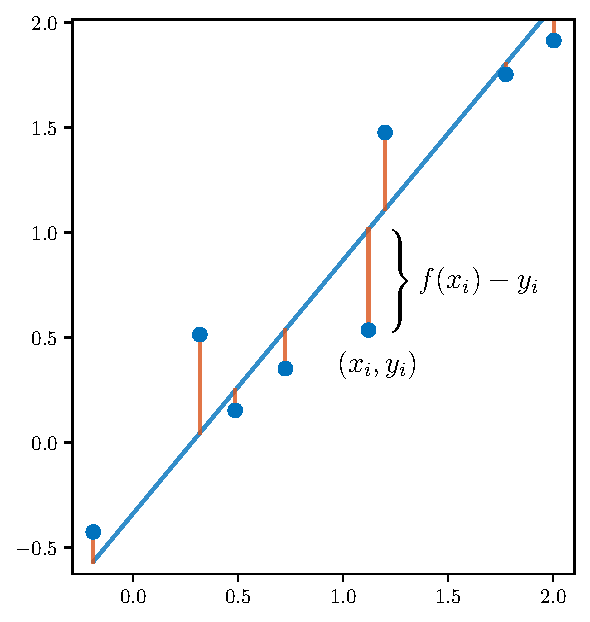
\includegraphics[width=.49\linewidth]{figs/fig-least-squares.pdf}
    \hfill
    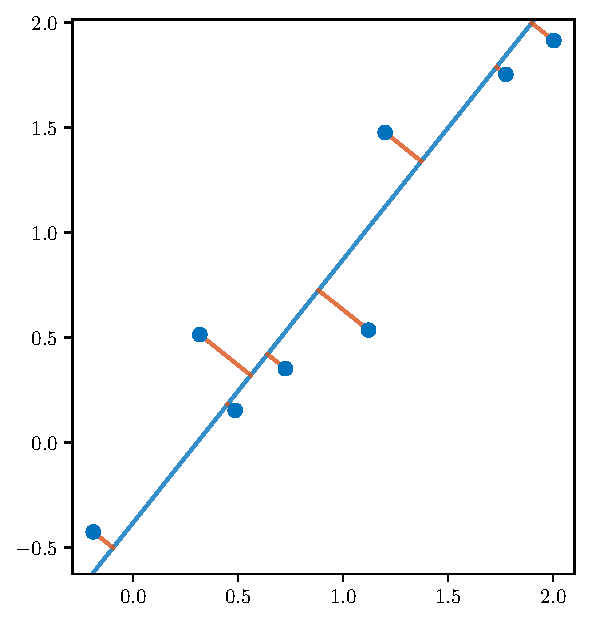
\includegraphics[width=.49\linewidth]{figs/fig-pca-fit.pdf}
    \caption{Least squares regression model \(f(x)\) (left) minimizes the sum of squared errors while total least squares, i.e., the PCA model \(g(x)\) (right) minimizes the orthogonal projections.}
    \label{fig:ols-pca}
\end{figure}
\end{example}